\documentclass[11pt]{article}
\usepackage{geometry}                % See geometry.pdf to learn the layout options. There are lots.
\geometry{letterpaper}                   % ... or a4paper or a5paper or ... 
%\geometry{landscape}                % Activate for for rotated page geometry
%\usepackage[parfill]{parskip}    % Activate to begin paragraphs with an empty line rather than an indent
\usepackage{graphicx}
\usepackage{amssymb}
\usepackage{amsmath}
\usepackage{epstopdf}
\usepackage{hyperref}
\DeclareGraphicsRule{.tif}{png}{.png}{`convert #1 `dirname #1`/`basename #1 .tif`.png}



\graphicspath{
{/Users/Andy/Cruises_Research/ChiPod/Cham_Eq14_Compare/mfiles/Patches/figures/}
}

\title{EQ14 - Computing gamma by patches}
\author{Andy Pickering}
%\date{}                                           % Activate to display a given date or no date



\begin{document}
\maketitle

\tableofcontents
\newpage




%~~~~~~~~~~~~~~~~~~~~~~~~~~~~~~~~~~~~~~~~~~~~~~~~~~~~~
%~~~~~~~~~~~~~~~~~~~~~~~~~~~~~~~~~~~~~~~~~~~~~~~~~~~~~
\section{Intro}

* These notes follow code \verb+Compute_gamma_by_patches.m+

In this analysis i'm tyring to compute $\Gamma$ for EQ14 Chameleon data by patch instead of just at every point. The equation used is 

\begin{equation}
\Gamma=\frac{N^2 \chi}{2\epsilon <dT/dz>^2}
\end{equation}

Figure \ref{gam_cham} shows the distribution of estimated gammas using all the chamleon data, and using just the data between 60 and 180m depth. The median gamma from both is about 0.02, about ten times smaller than the usually assumed $\Gamma=0.2$.

\begin{figure}[htbp]
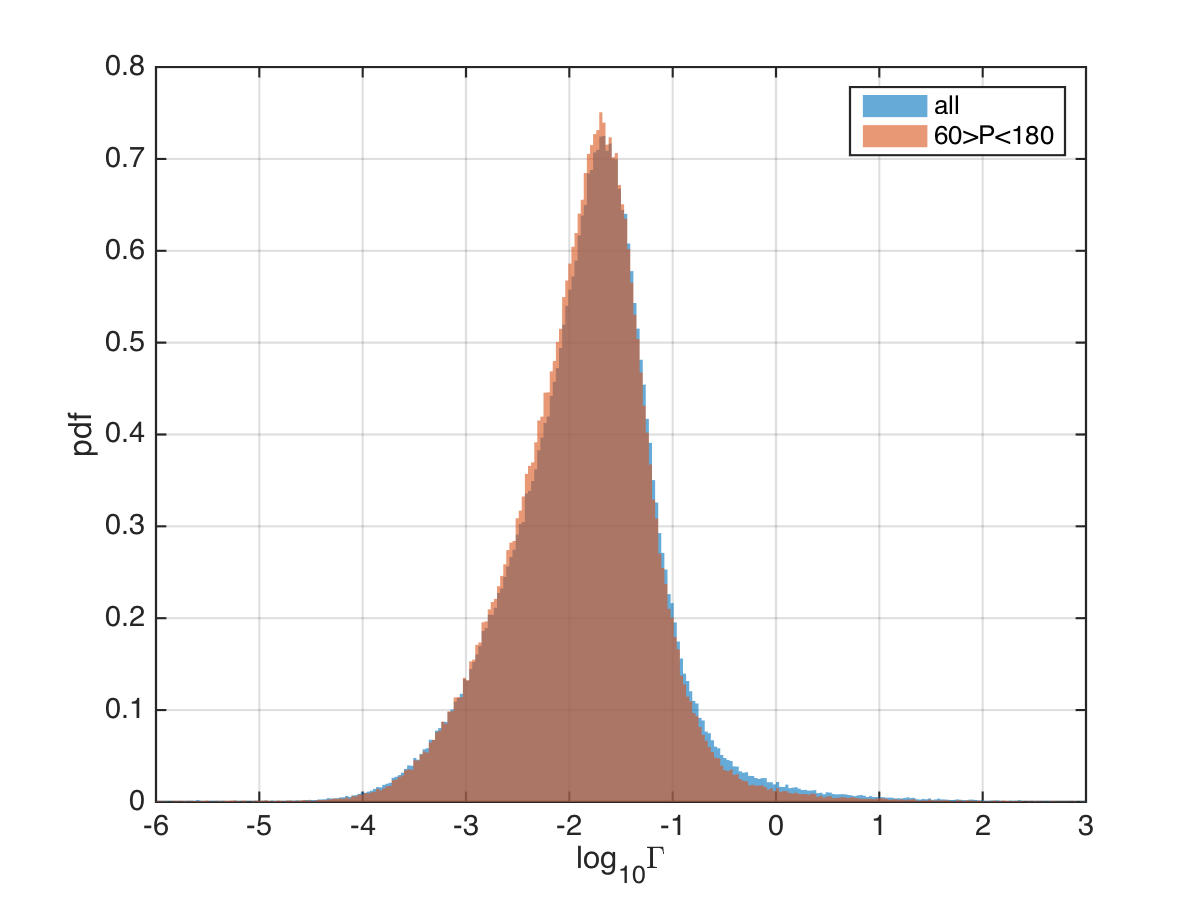
\includegraphics[scale=0.8]{gam_cham_hist.png}
\caption{Histogram of $\Gamma$ for all EQ14 chameleon profiles.}
\label{gam_cham}
\end{figure}




\clearpage
%~~~~~~~~~~~~~~~~~~~~~~~~~~~~~~~~~~~~~~~~~~~~~~~~~~~~~
%~~~~~~~~~~~~~~~~~~~~~~~~~~~~~~~~~~~~~~~~~~~~~~~~~~~~~
\section{ Looking at stratification etc.}

Looking in more detail at relationships between straitifcation, $\chi$, and $\Gamma$ as suggested by Emily. See \verb+MakeEmilysPlot.m+. Figure \ref{2x2hist} shows 2-D histograms of gamma vs each variable. Figure \ref{gambychin2} shows the mean and median values of gamma for bins of chi vs N2.


\begin{figure}[htbp]
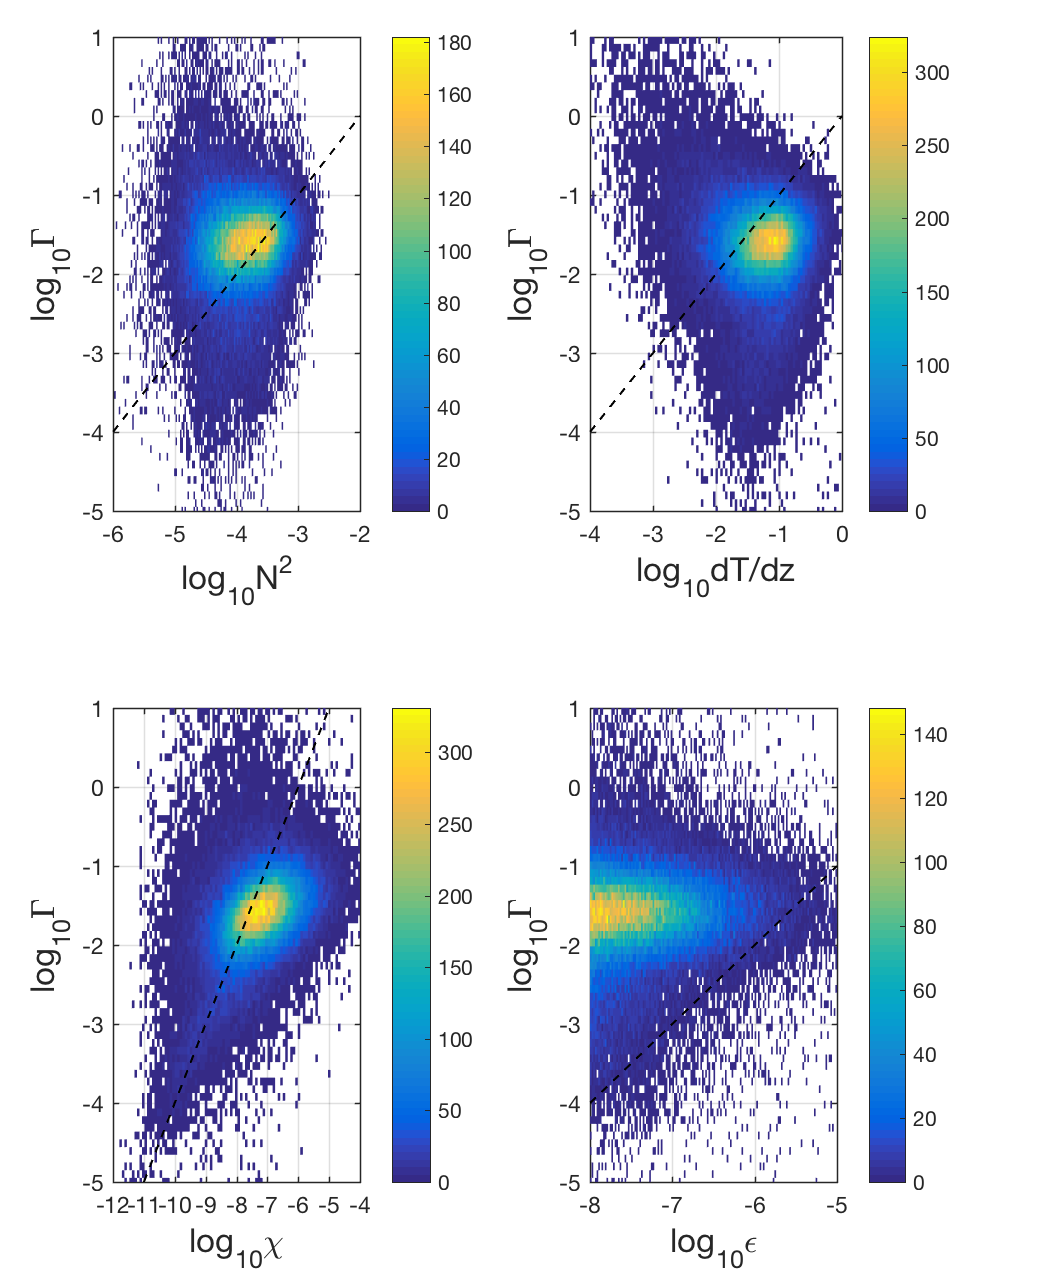
\includegraphics[scale=0.8]{2X2_2dhist_Gamma.png}
\caption{2-D histograms of $\Gamma$ vs each variable. Black line shows 1:1 relationship.}
\label{2x2hist}
\end{figure}


\begin{figure}[htbp]
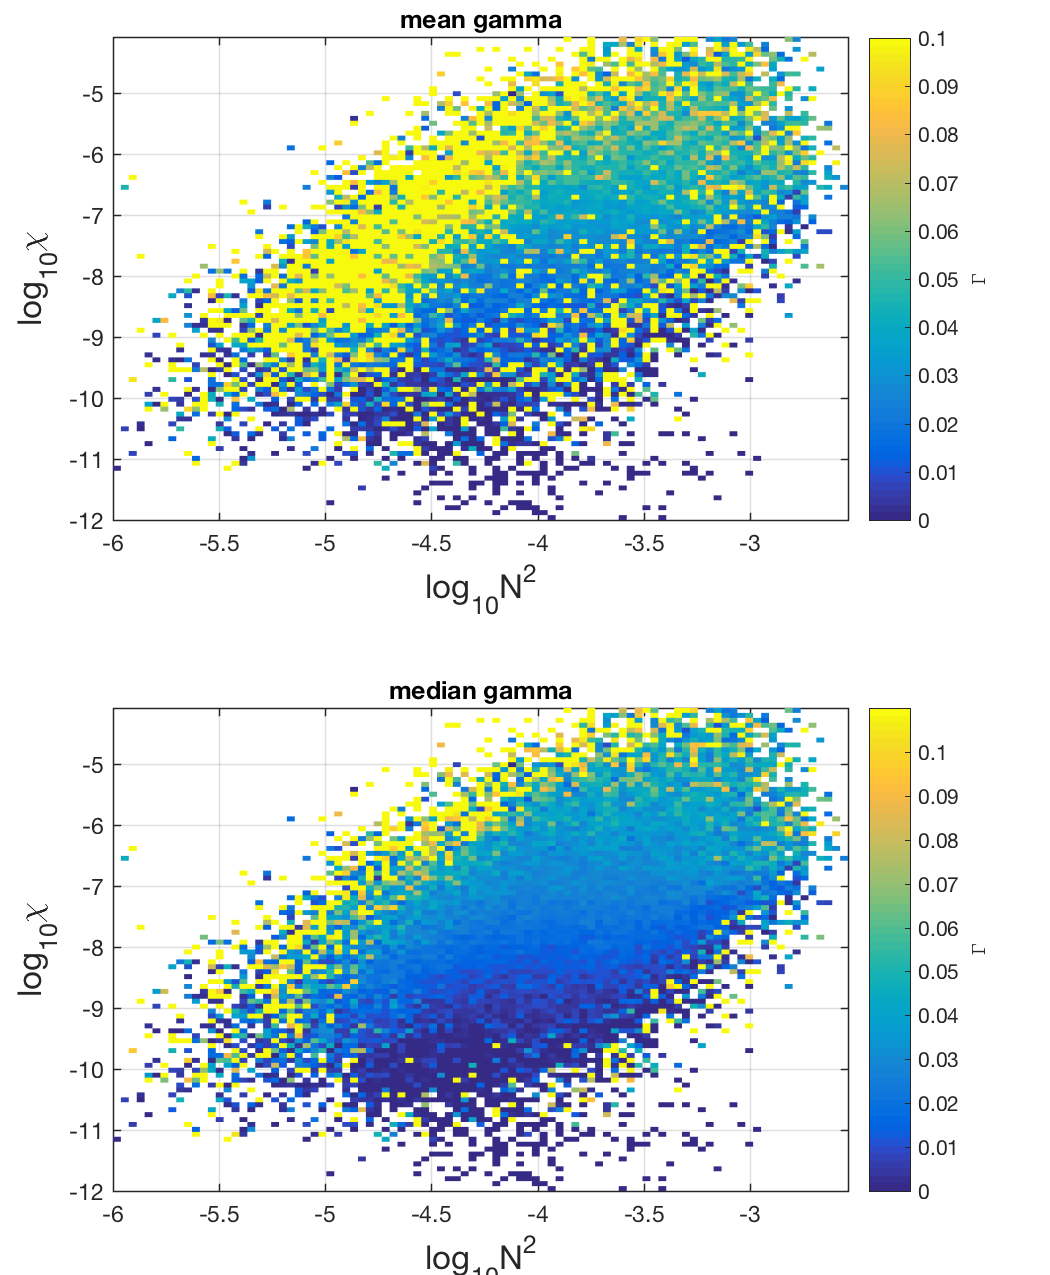
\includegraphics[scale=0.8]{Gamma_binnedBy_N2_chi.png}
\caption{Mean (top) and median (bottom) values of gamma computed for bins of $\chi$ and $N^2$.}
\label{gambychin2}
\end{figure}





\clearpage
%~~~~~~~~~~~~~~~~~~~~~~~~~~~~~~~~~~~~~~~~~~~~~~~~~~~~~
%~~~~~~~~~~~~~~~~~~~~~~~~~~~~~~~~~~~~~~~~~~~~~~~~~~~~~
\section{Identifying Patches}

I first identify patches (overturns) using potnential density computed from 1m binned temperature and salinity from Chameleon profiles. This is dones w/ \verb+IdentifyPatches.m+.

\begin{itemize}
\item Figure \ref{psizebox} shows the distribution of patch sizes from all profiles (exluding those above 20m and below 180m). Only about 11\% of the orginal patches are in this good depth range. Most of the patches are very small (1-2m).
\item Figure \ref{epswot} shows $\epsilon$ with overturn locations plotted over. The majority of the identified overturns occur between 20-60m, associated with the diurnal cycle of turbulence. These probably shouldn't even be included in the chipod analysis since the assumed dynamics do not hold.
\item Below that, overturns generally co-occur with larger $\epsilon$ measured by chameleon shear probe. There are some that occur where chameleon $\epsilon$ is small, however.
\item Figure \ref{hists_allVspatch} shows distributions of all data versus just data within the identified patches. Patches are associated with lower N2 and dtdz, and higher epsilon. The distribution of chi does not appear to be significantly different.
\end{itemize}


\begin{figure}[htbp]
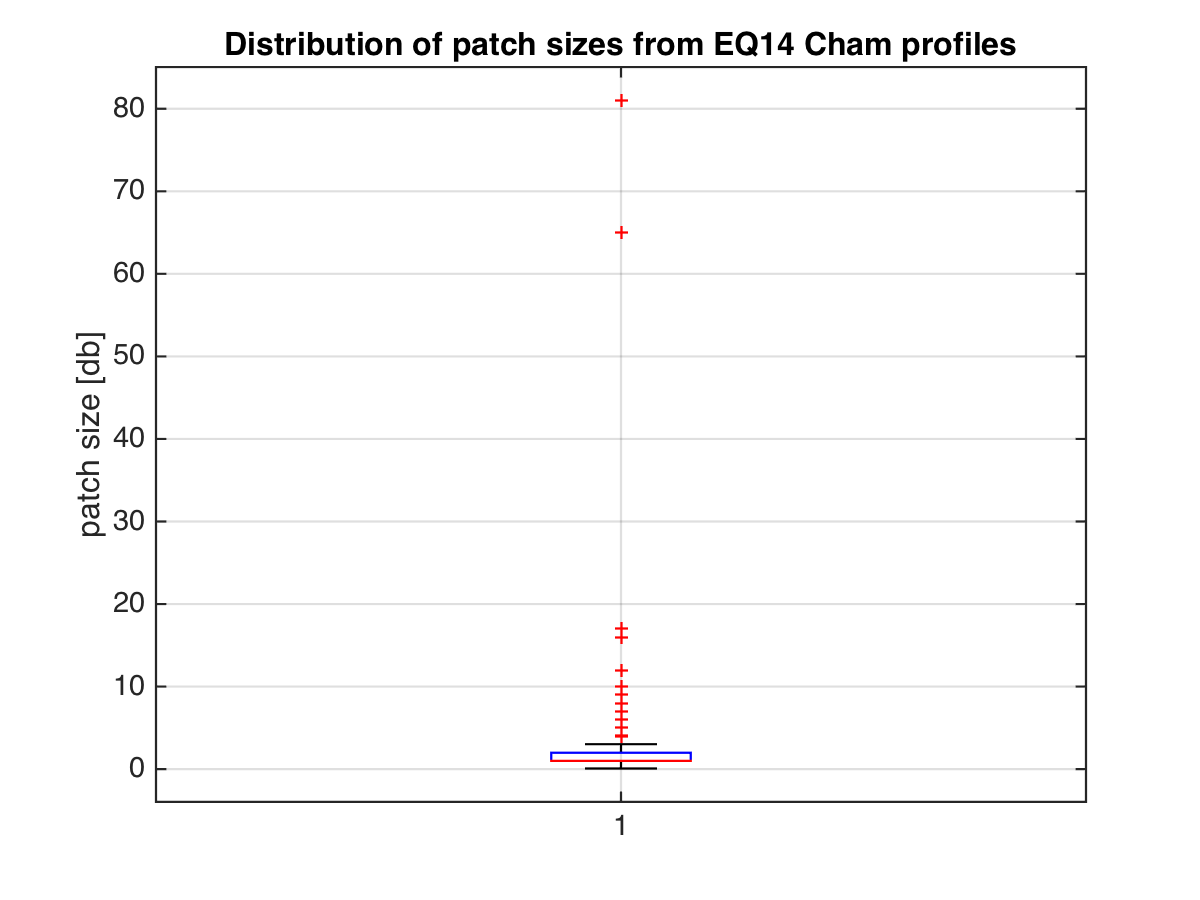
\includegraphics[scale=0.8]{GamByPatch_patchsize_boxplot.png}
\caption{Boxplot of the patch sizes for all EQ14 chameleon profiles. Only patches occuring at depths between 20 and 180 m are considered.}
\label{psizebox}
\end{figure}

\begin{figure}[htbp]
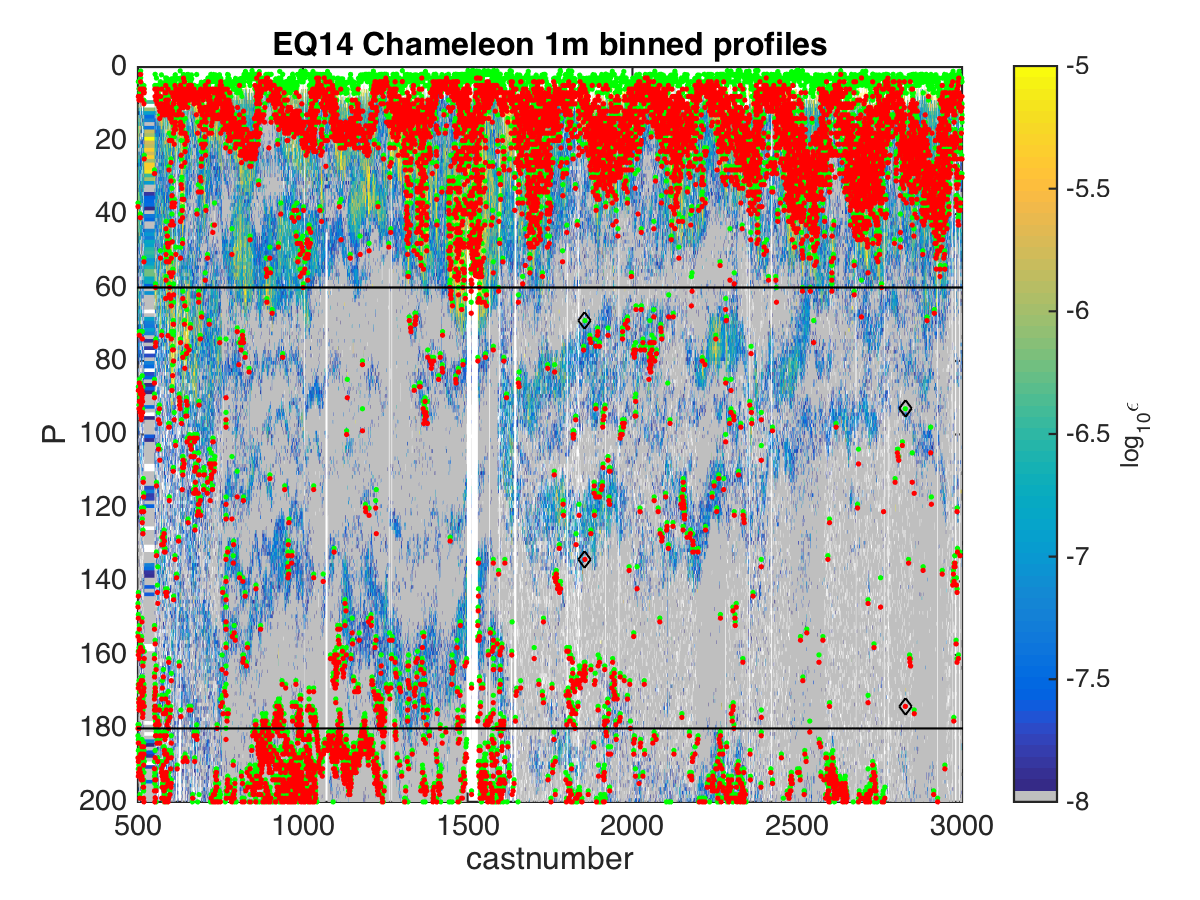
\includegraphics[scale=0.8]{GamByPatch_eps_pcolor_wpatches.png}
\caption{$\epsilon$ measured by chameleon shear probes on EQ14 profiles. Identified overturns are plotted in green/red. Black diamonds indicate overturns larger than 20m, these are ignored (there are only 2).}
\label{epswot}
\end{figure}

\begin{figure}[htbp]
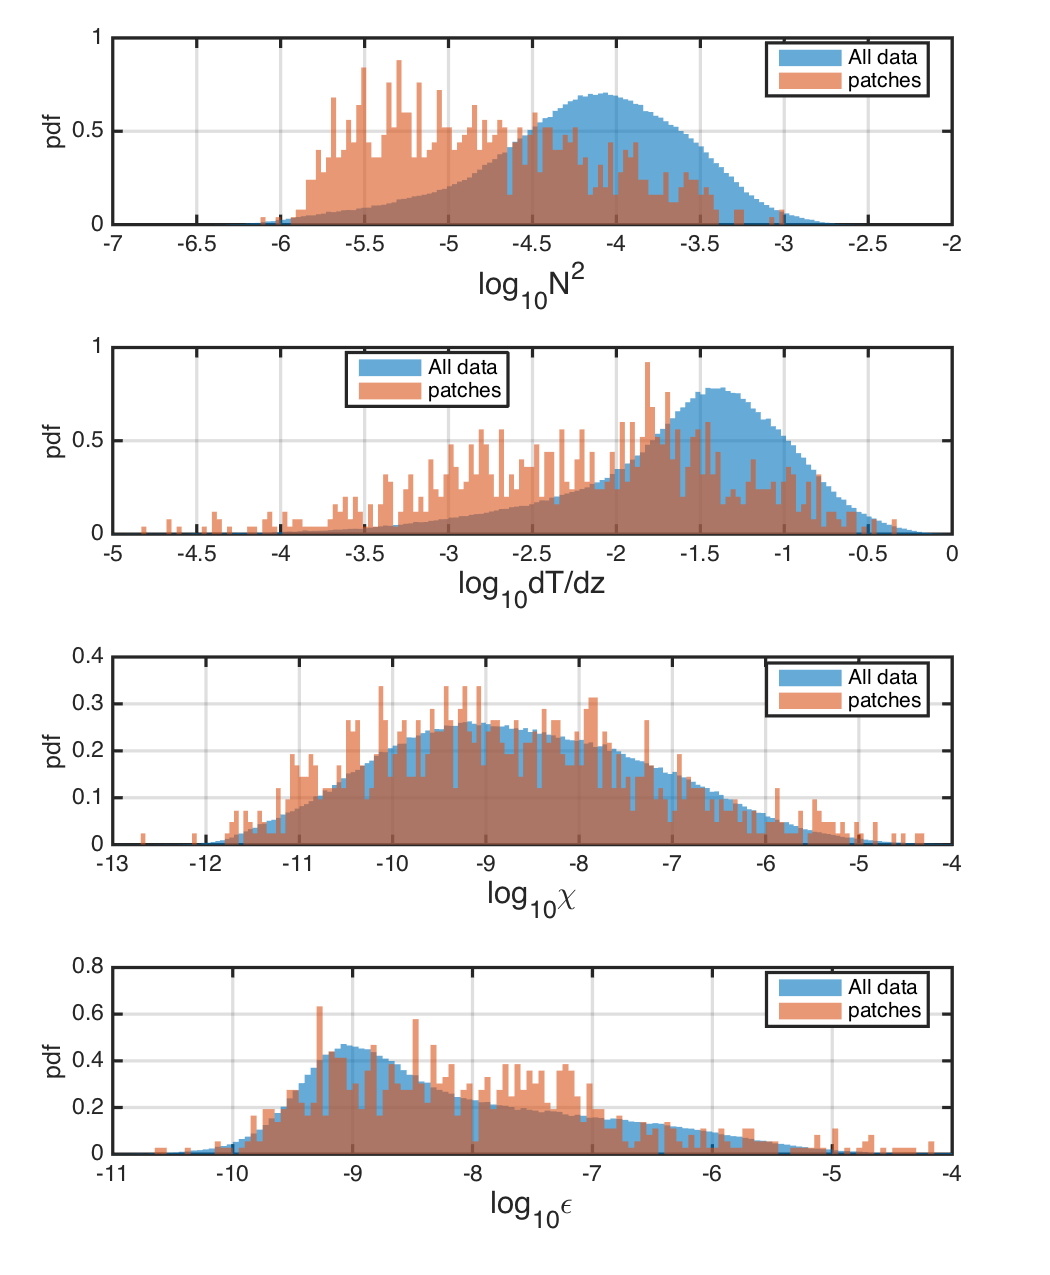
\includegraphics[scale=0.8]{hists_allVspatch.png}
\caption{Distributions of N2,dtdz,chi,eps from EQ14 chameleon profiles, for all data and just within patches.}
\label{hists_allVspatch}
\end{figure}


\clearpage
%~~~~~~~~~~~~~~~~~~~~~~~~~~~~~~~~~~~~~~~~~~~~~~~~~~~~~
%~~~~~~~~~~~~~~~~~~~~~~~~~~~~~~~~~~~~~~~~~~~~~~~~~~~~~
\section{Computing gamma by patch}

The next step is to compute $\Gamma$ over each patch. I will use $N^2$ and $dT/dz$ averaged over the patch (since most patches are very small, this probably won't differ too much?). For $\chi$ and $\epsilon$, I should compute these from spectra over the entire patch. This will involve hacking into the chameleon processing codes a bit... Before I do this, I will try just using the 1m binned values within each patch.

So far this doesn't seem to be giving me anything close to $\Gamma=0.2$ (figure \ref{hists_gamma_allVspatch}). Figure \ref{gamvspatchsize} shows gamma plotted vs patch size. It seems like the maximum gamma decreases linearly with patch size. We can also see that gamma is dominated by a very large number of small values, especially for smaller patch sizes.

\begin{figure}[htbp]
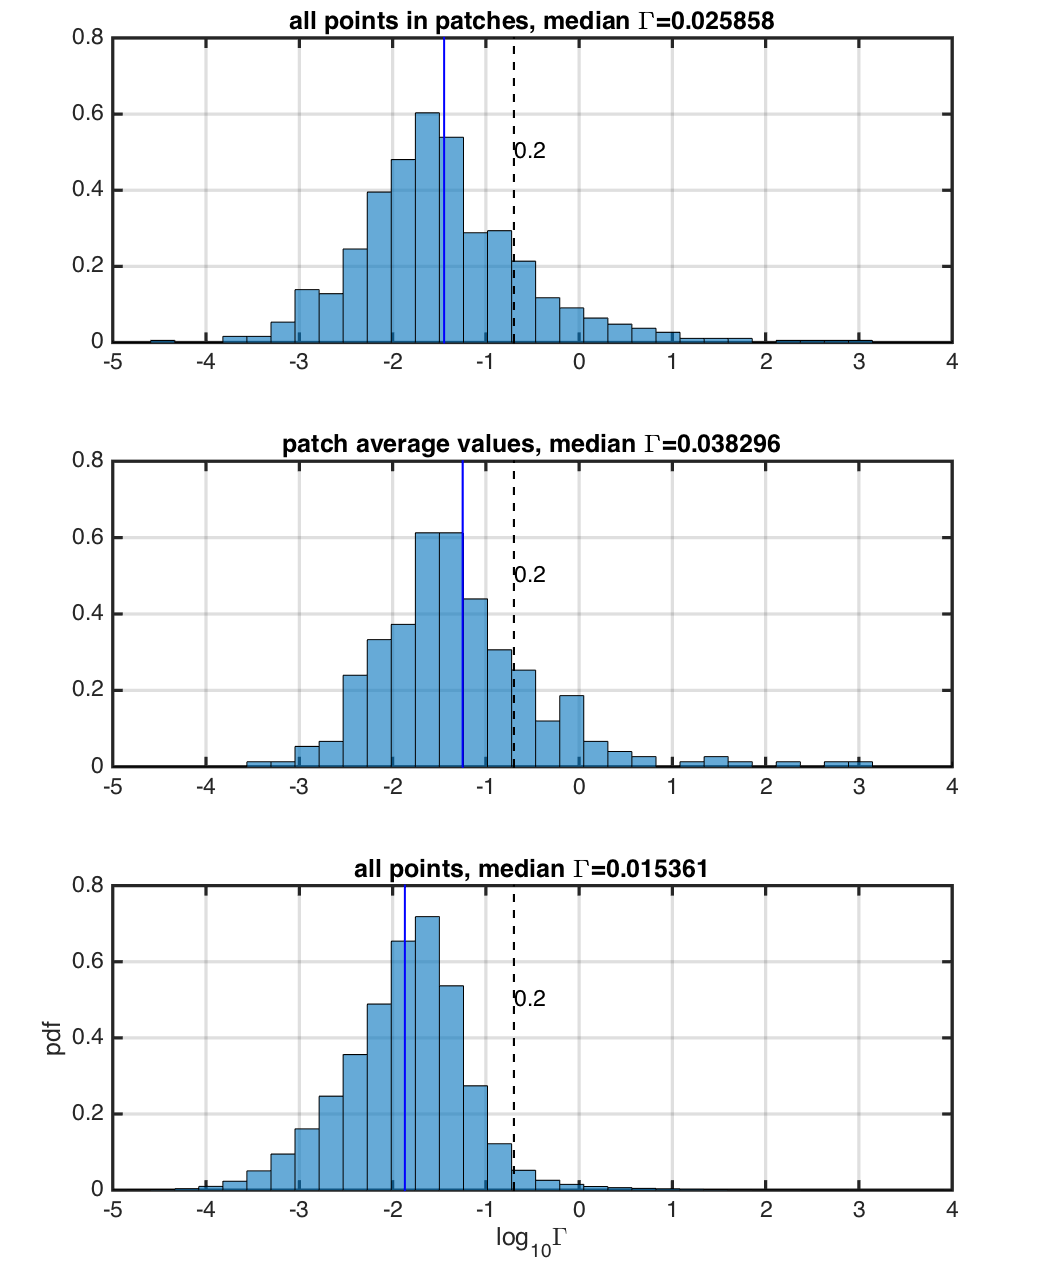
\includegraphics[scale=0.8]{hists_gamma_allVspatch.png}
\caption{Histograms of gamma for (1) all points within patches (2) using averaged values from patches (3) using all points. Only data between 60-180m depth is used for all.  Blue line shows median of each distribution, and black dashed line is 0.2.}
\label{hists_gamma_allVspatch}
\end{figure}

\begin{figure}[htbp]
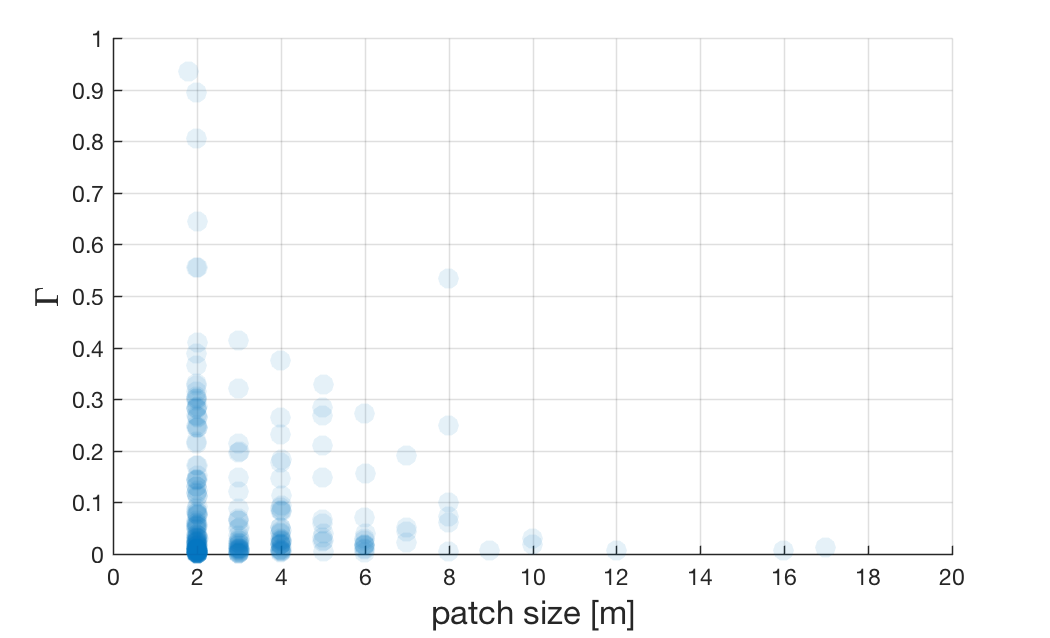
\includegraphics[scale=0.8]{gamma_Vs_patchsize.png}
\caption{Scatter plot of gamma vs patch size for EQ14 profiles.}
\label{gamvspatchsize}
\end{figure}




\clearpage
%~~~~~~~~~~~~~~~~~~~~~~~~~~~~~~~~~~~~~~~~~~~~~~~~~~~~~
%~~~~~~~~~~~~~~~~~~~~~~~~~~~~~~~~~~~~~~~~~~~~~~~~~~~~~
\section{TIWE Patches from Bill}

See \verb+LookAt_TIWE_Data_Bill.m+. Bill sent data from TIWE patches (patches computed by Doug Caldwell?), I saved them in \verb+/ChiPod/TIWE/events_TIWE.mat/+.

\begin{figure}[htbp]
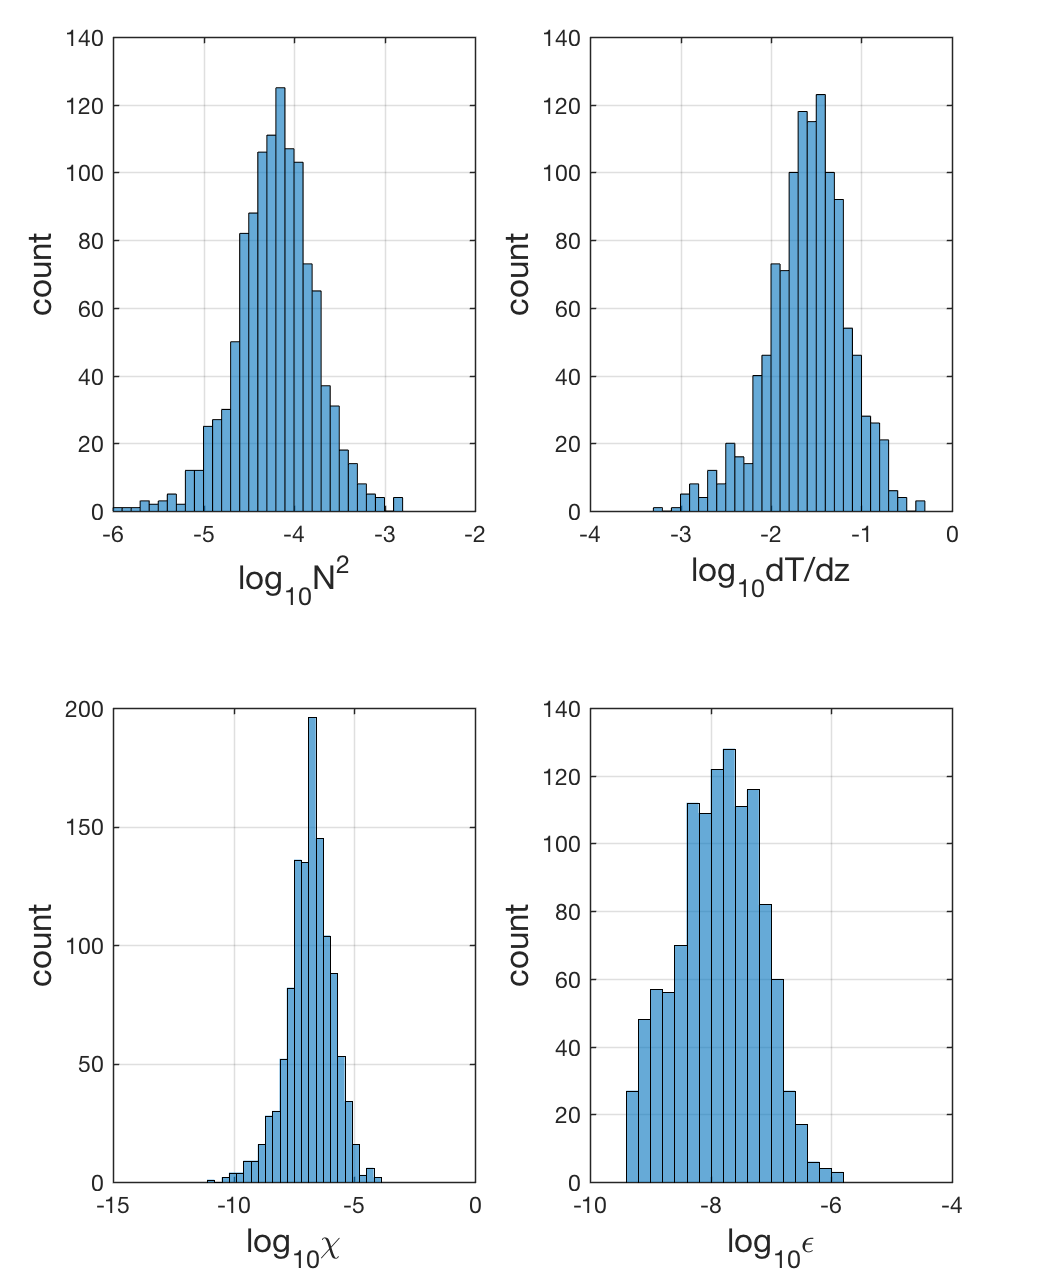
\includegraphics[scale=0.8]{tiwe_patches_bill_hist.png}
\caption{Histograms of data from Bill's tiwe patches.}
\label{}
\end{figure}

\begin{figure}[htbp]
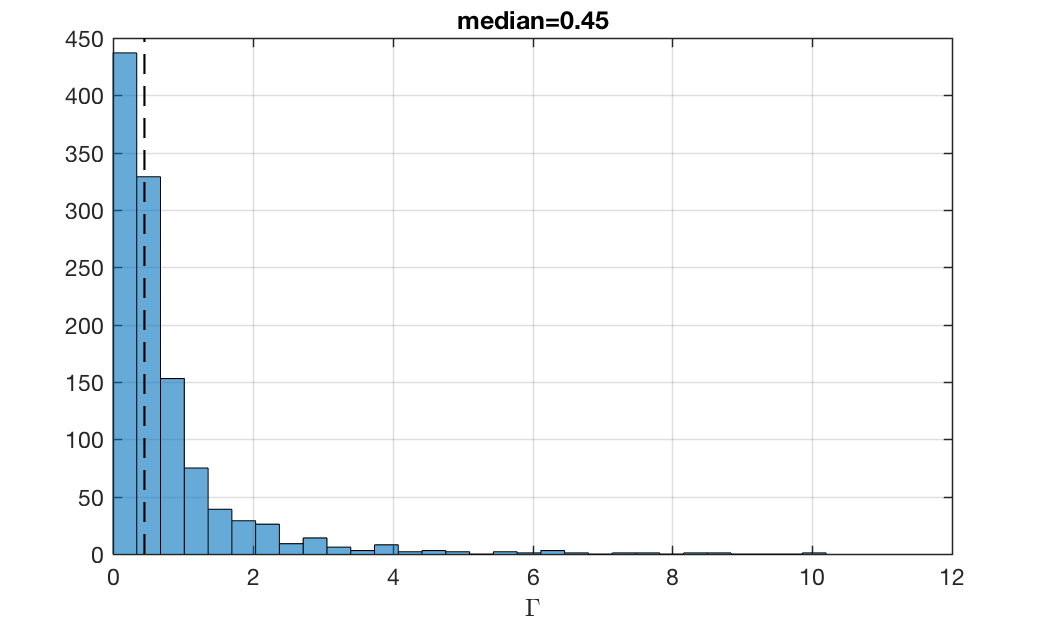
\includegraphics[scale=0.8]{tiwe_patches_bill_hist_gam.png}
\caption{Histograms of gamma computed w/ data from Bill's tiwe patches.}
\label{}
\end{figure}



\clearpage
%~~~~~~~~~~~~~~~~~~~~~~~~~~~~~~~~~~~~~~~~~~~~~~~~~~~~~
%~~~~~~~~~~~~~~~~~~~~~~~~~~~~~~~~~~~~~~~~~~~~~~~~~~~~~
\section{FLX91 Patches}

Jim and Bill both sent their patch data from flx91 also. I saved these as \newline \verb+ChiPod/Flux91/flx91_patch_out_nov94.mat+ and  \newline \verb+ChiPod/Flux91/events_FLX91.mat+. \newline

See \verb+LookAtFlux91Data_Jim.m+, \verb+LookAtFlux91Data_Bill.m+, \verb+Compare_tiwe_patches_jim_bill.m+. \newline

Summary:
\begin{itemize}
\item Distributions of n2, dtdz, chi, eps look a little different. Jim's data seem to contain larger values of all variables.
\item But distributions of gamma look similar. Both have medians around 0.3 .
\item The data is very old and codes used to compute patches not available, so it is difficult for me to reproduce the analysis or apply my own analysis to the raw data and compare.
\end{itemize}


%~~~~~~~~~~
\subsection{Jim}

\begin{figure}[htbp]
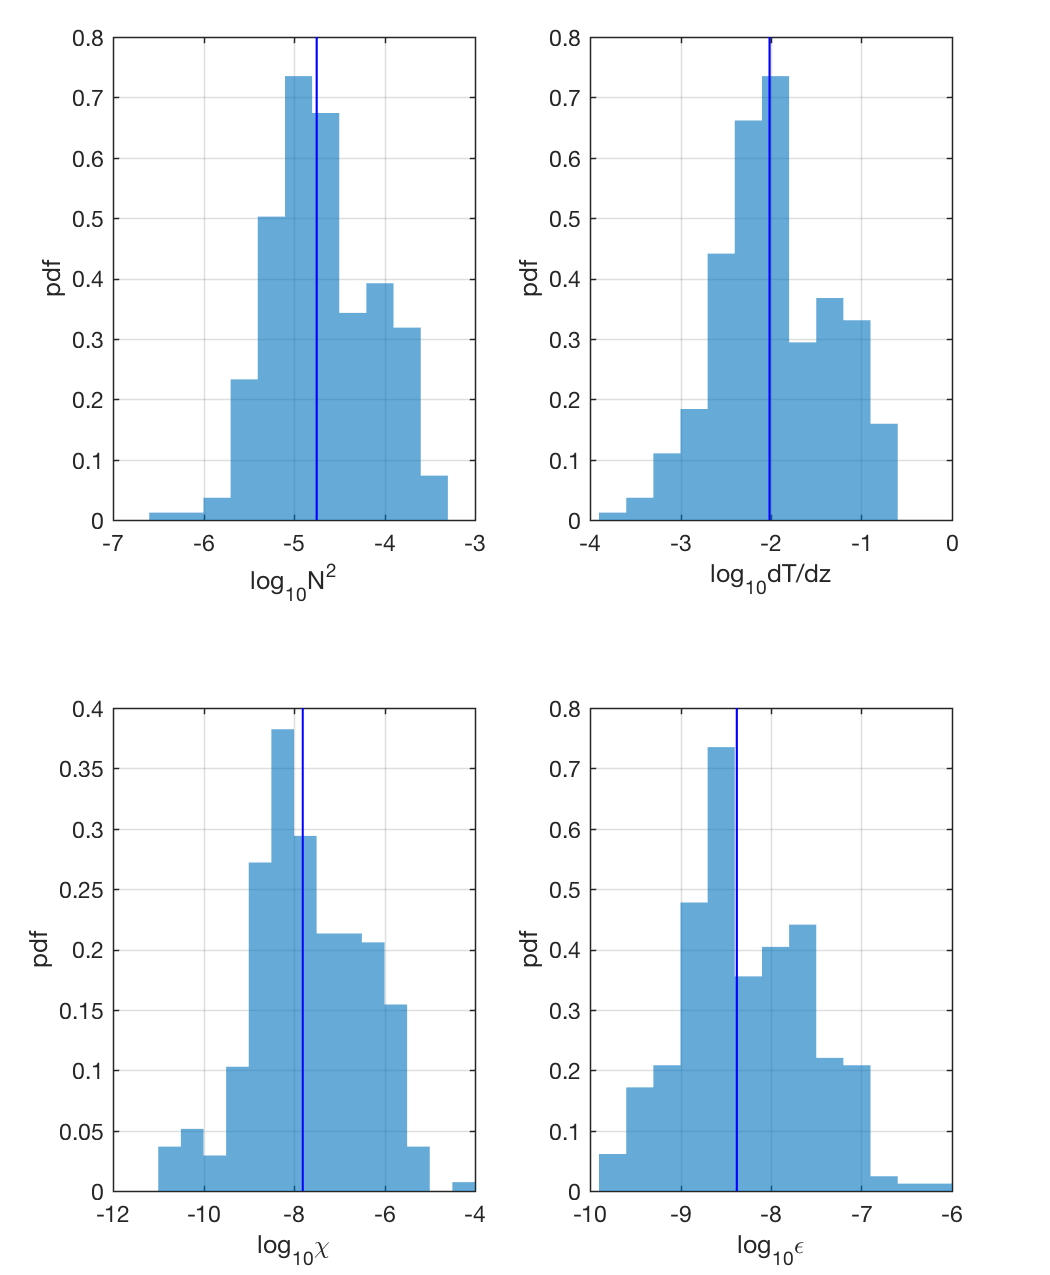
\includegraphics[scale=0.8]{flx91_patches_jim_hist.png}
\caption{Histograms of data from Jim's flx91 patches. Vertical lines show median.}
\label{}
\end{figure}

\begin{figure}[htbp]
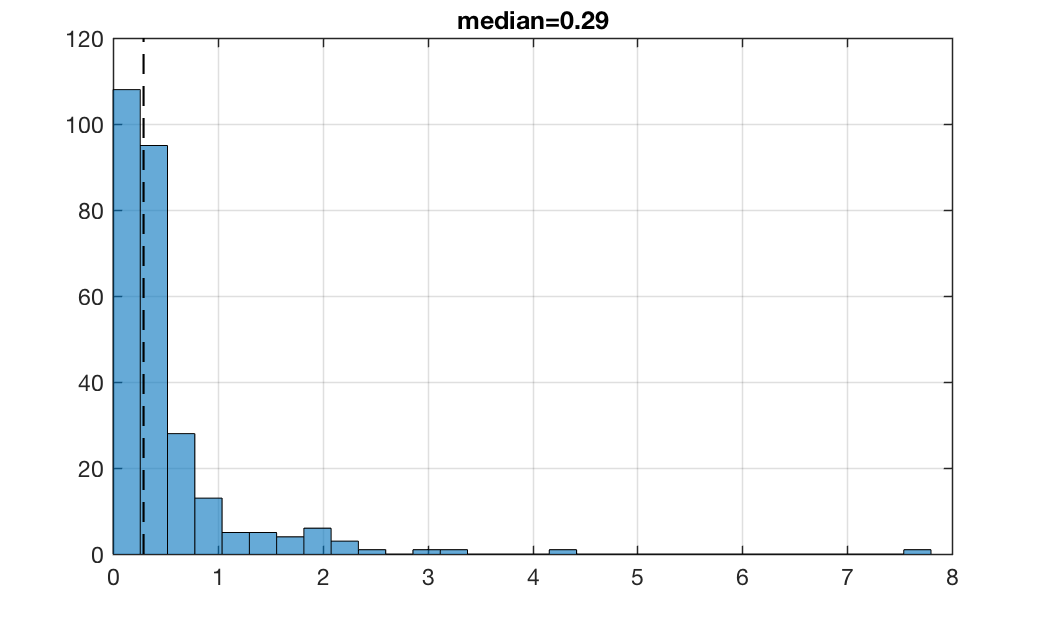
\includegraphics[scale=0.8]{flx91_patches_jim_hist_gam.png}
\caption{Histograms of gamma computed w/ data from Jim's flx91 patches.}
\label{}
\end{figure}

%~~~~~~~~~~
\subsection{Bill}

\begin{figure}[htbp]
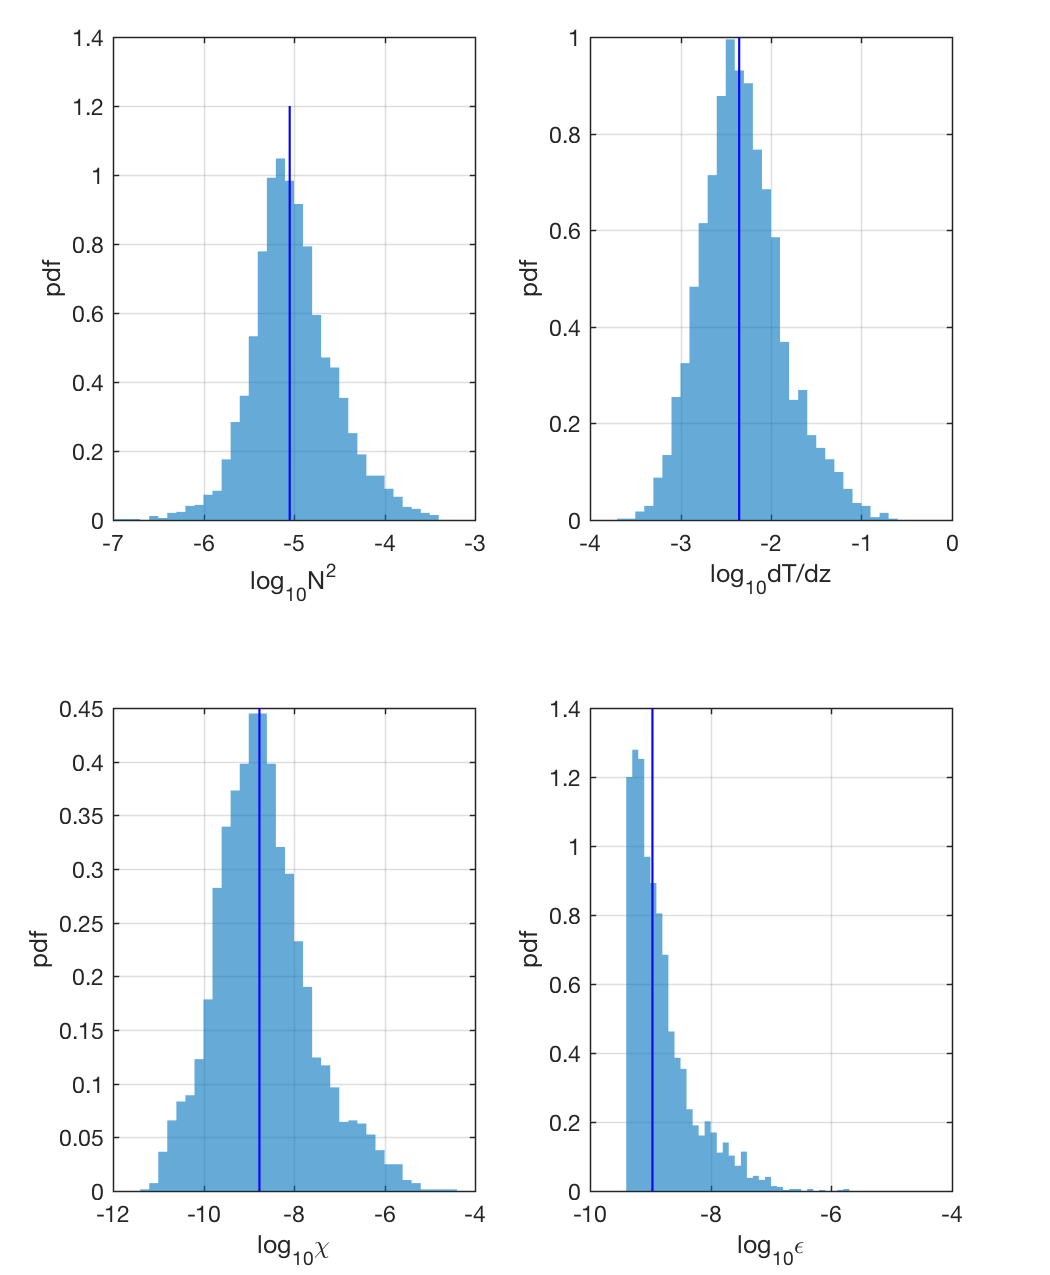
\includegraphics[scale=0.8]{flx91_patches_Bill_hist.png}
\caption{Histograms of data from Bill's flx91 patches. Vertical lines show median.}
\label{}
\end{figure}

\begin{figure}[htbp]
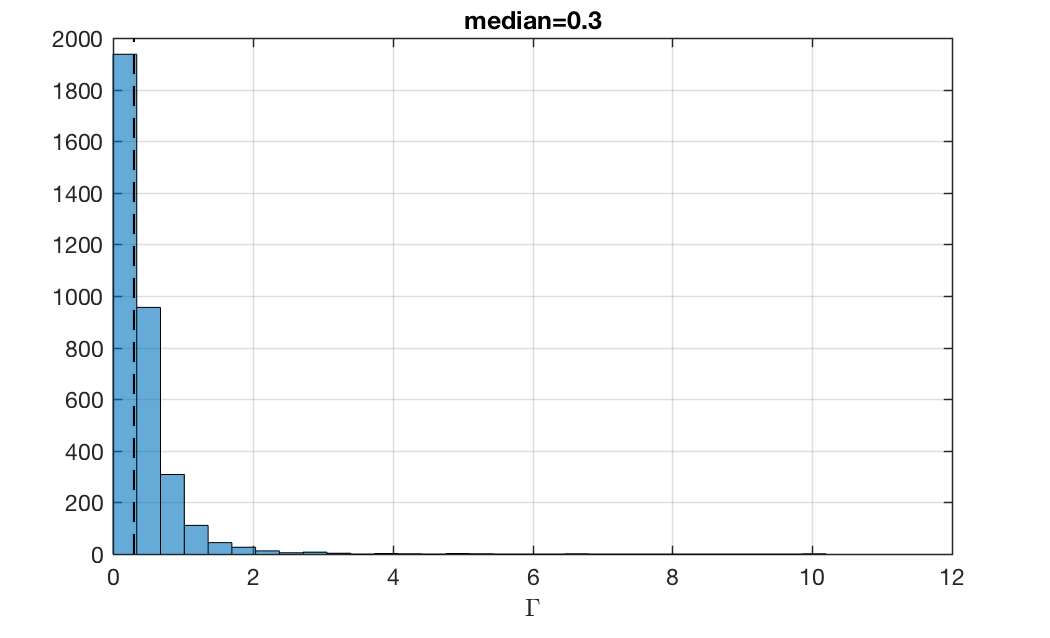
\includegraphics[scale=0.8]{flx91_patches_Bill_hist_gam.png}
\caption{Histograms of gamma computed w/ data from Bill's flx91 patches.}
\label{}
\end{figure}


%~~~~~~~~~~
\subsection{Comparison}


\begin{figure}[htbp]
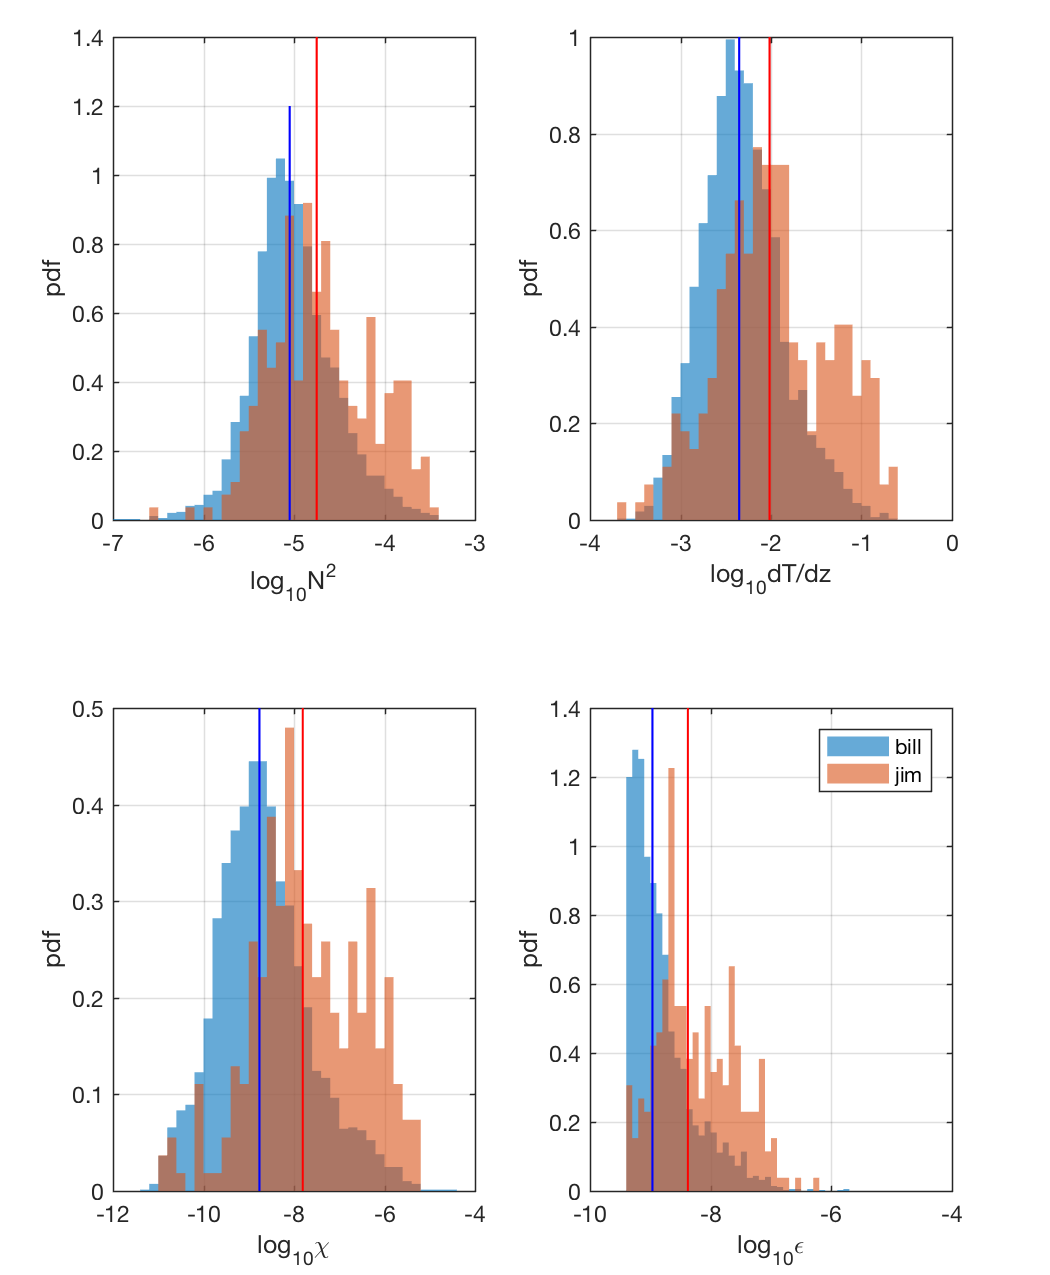
\includegraphics[scale=0.8]{flx91_hist_compare_bill_jim.png}
\caption{Histograms computed w/ data from Bill and Jim's flx91 patches.}
\label{}
\end{figure}



\begin{figure}[htbp]
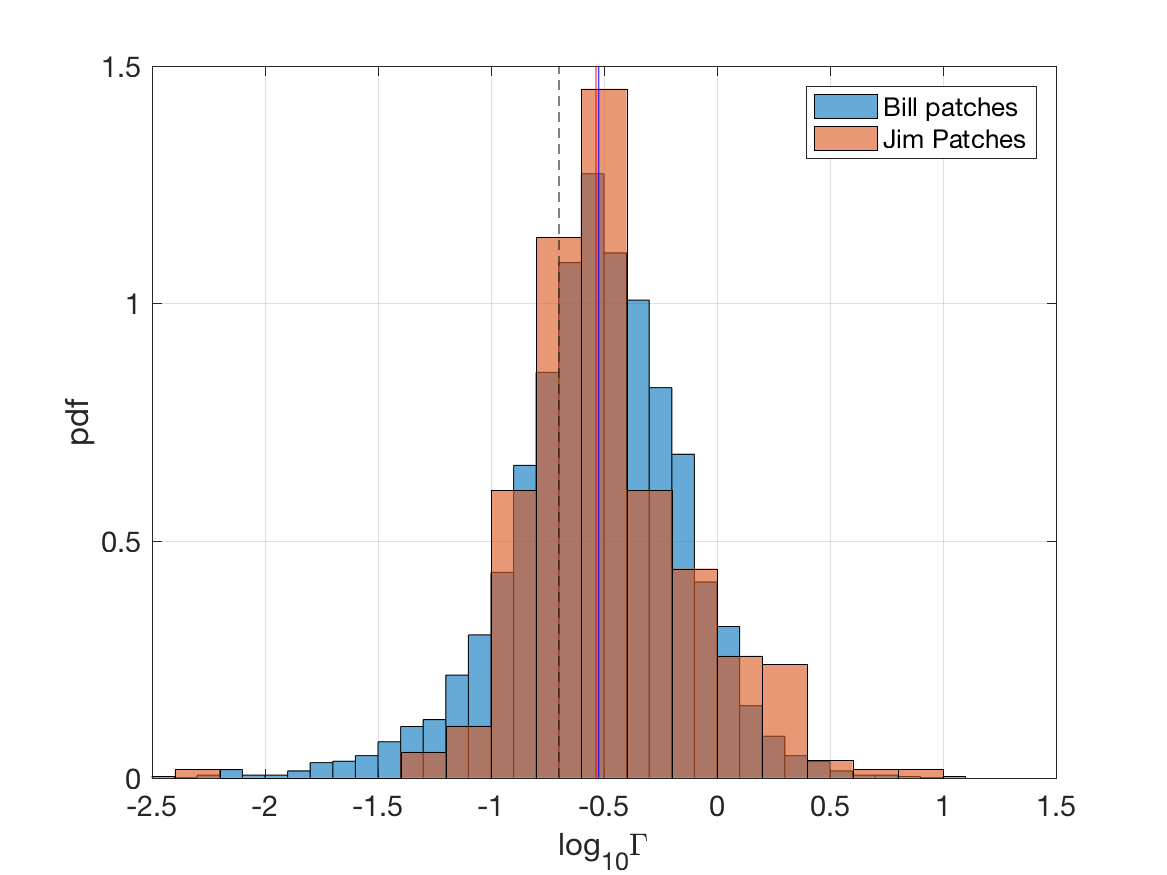
\includegraphics[scale=0.8]{flx91_gam_hist_compare_bill_jim.png}
\caption{Histograms of gamma computed w/ data from Bill and Jim's flx91 patches.}
\label{}
\end{figure}






\clearpage
%~~~~~~~~~~~~~~~~~~~~~~~~~~~~~~~~~~~~~~~~~~~~~~~~~~~~~
%~~~~~~~~~~~~~~~~~~~~~~~~~~~~~~~~~~~~~~~~~~~~~~~~~~~~~
\section{TIWE Comparisons}

Jonathan shared the entire TIWE folder (from Ganges I think?) with me on Dropbox. There are a lot of different folders/versions. 
I�m going to try using the processed mat files for each cast in \verb+Tiwe91/mat_Greg_analysis/+.

I first combine all the profiles in \verb+Combine_TIWE.m+, interpolating each profile onto the same depth vector w/ 1m spacing. Figure \ref{tiwe_comb} shows data from all the combined profiles. Note that something seems weird with dT/dz; many profiles have a constant near-zero dTdz below 150m.  Other than that, the data look qualitatively similar to EQ14.


\begin{figure}[htbp]
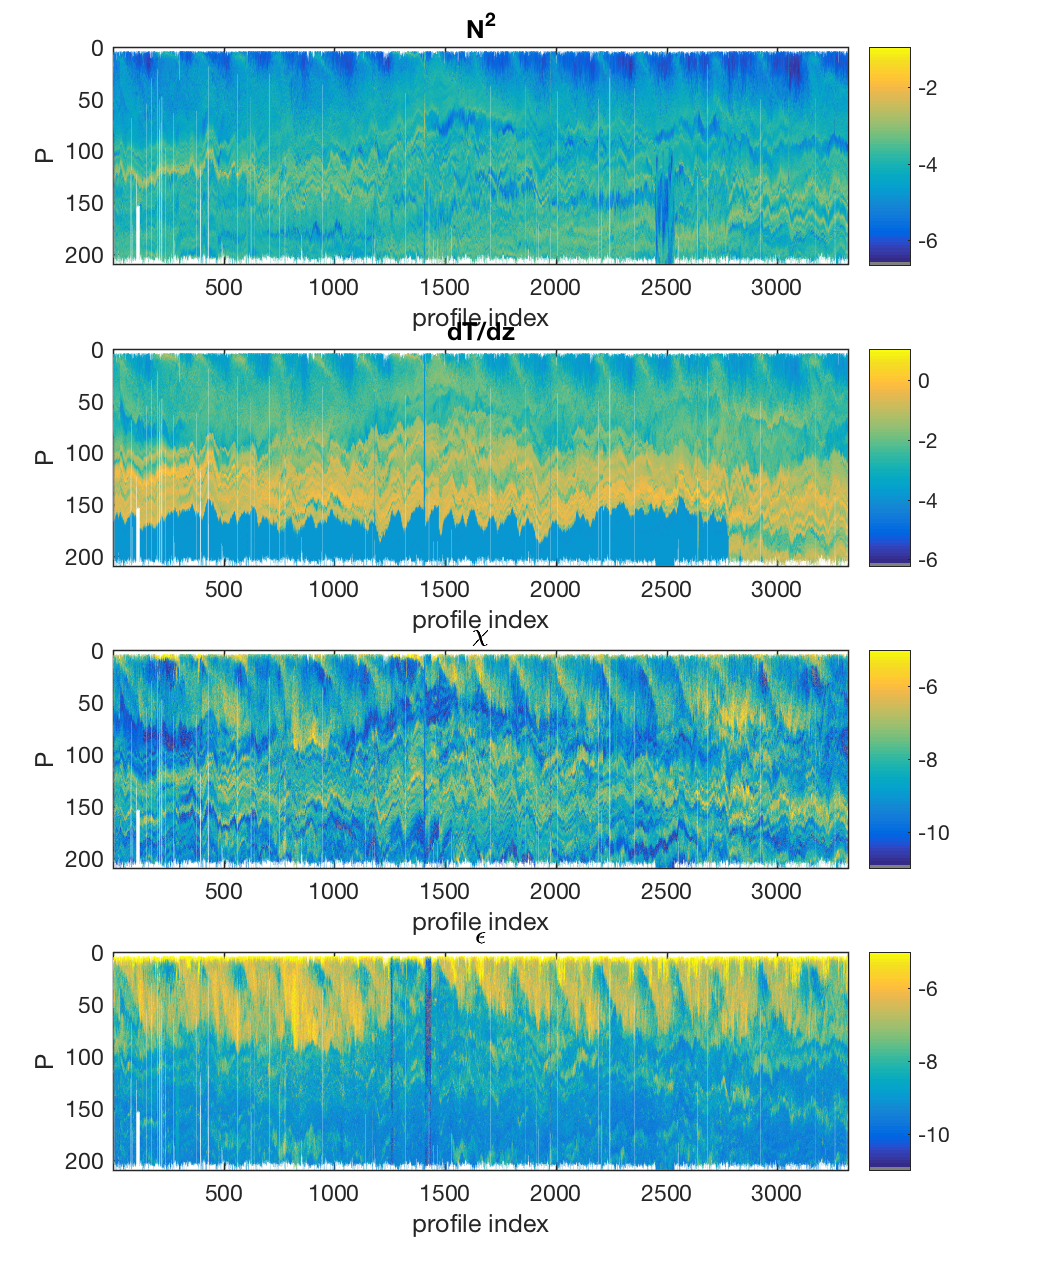
\includegraphics[scale=0.8]{tiwe_comb_n2_dtdz_chi_eps.png}
\caption{N2,dtdz,chi, and eps from combined TIWE data.}
\label{tiwe_comb}
\end{figure}
\clearpage

Next i'll compare the distributions of each variable to the EQ14 data (Figure \ref{tiwe_eq14_comp}). N2 and epsilon look very similar. Chi from tiwe is a bit narrower but they have similar medians. Dt/dz from tiwe has a spike at those weird small values, and then a sort of two-peak distribution. Figure \ref{tiwe_eq14_comp_fix} shows the same plots with the bad dtdz values removed.L


\begin{figure}[htbp]
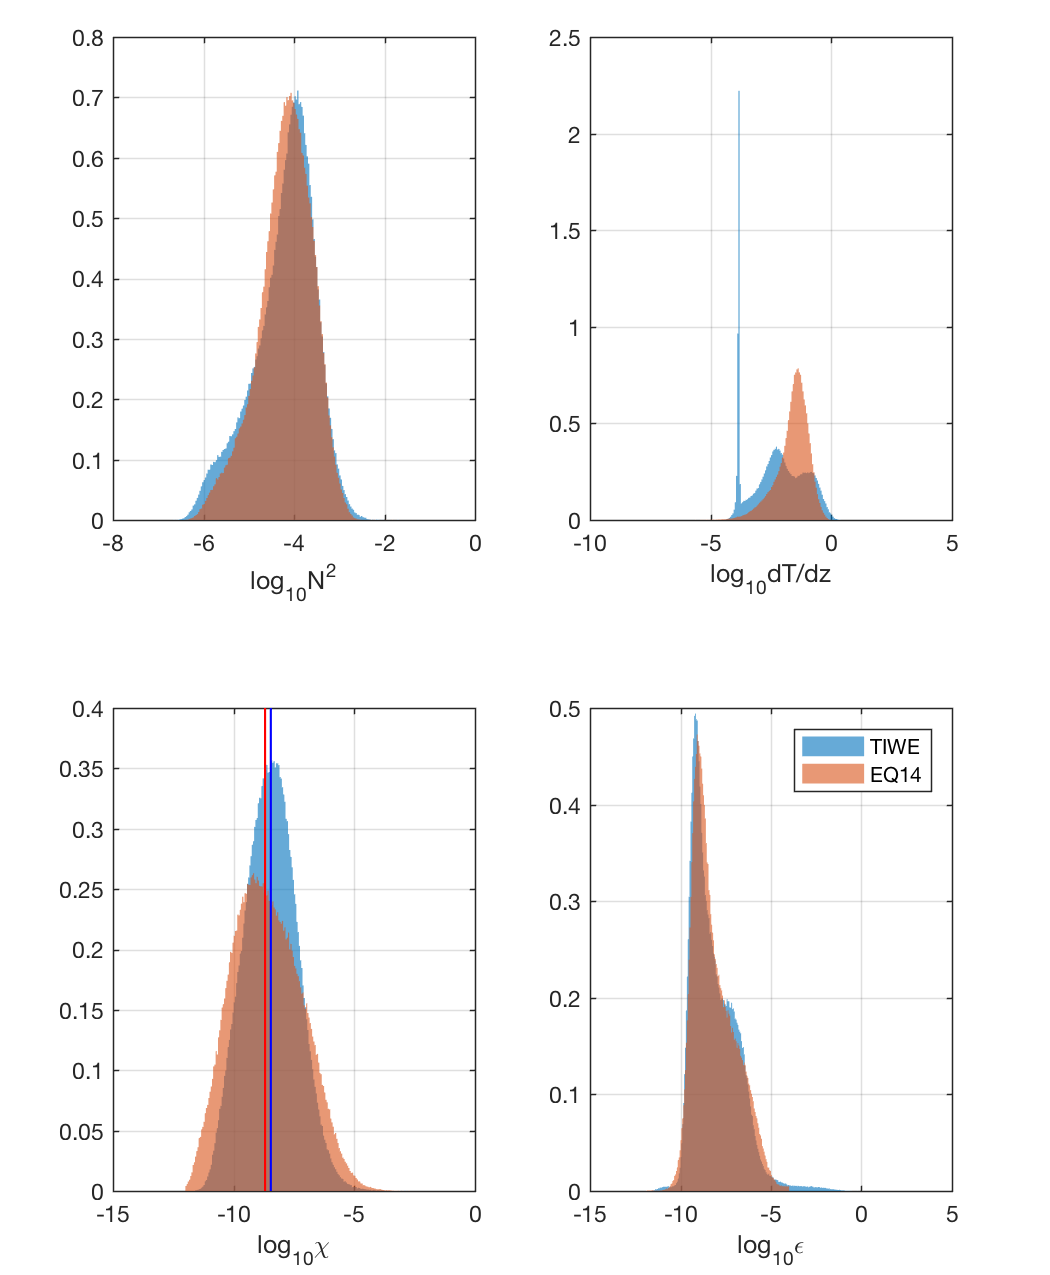
\includegraphics[scale=0.8]{tiwe_eq14_hist_compare.png}
\caption{Histograms of N2,dtdz,chi, and eps from combined TIWE data and EQ14 data.}
\label{tiwe_eq14_comp}
\end{figure}

\begin{figure}[htbp]
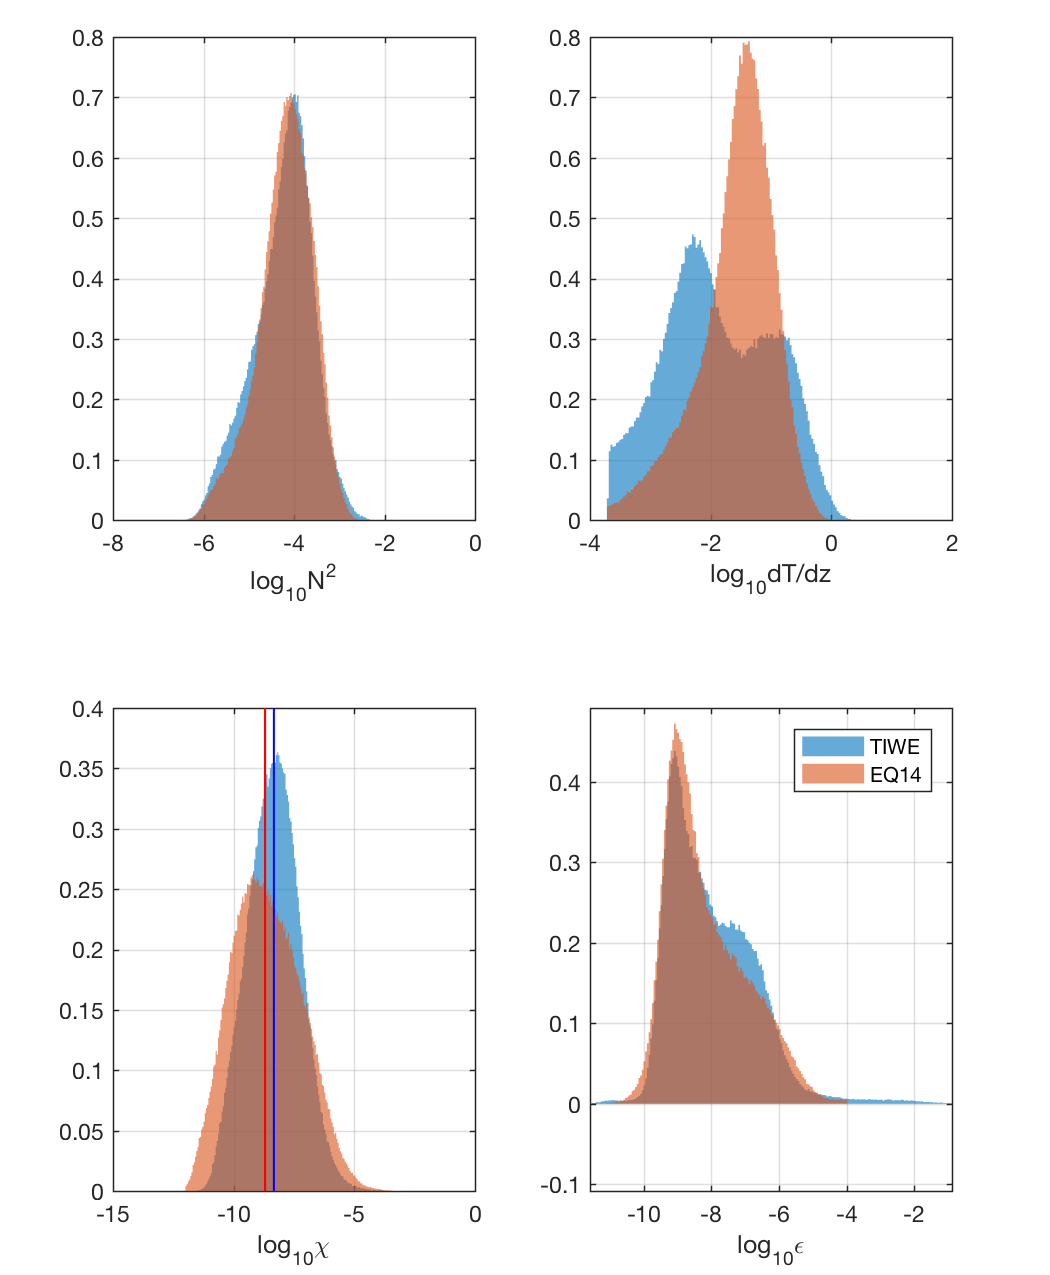
\includegraphics[scale=0.8]{tiwe_eq14_hist_compare_fixdtdz.png}
\caption{Histograms of N2,dtdz,chi, and eps from combined TIWE data and EQ14 data, with bad dT/dz values not included.}
\label{tiwe_eq14_comp_fix}
\end{figure}

\clearpage


\subsection{Gamma}
What does gamma look like for the tiwe data? Figure \ref{tiwe_eq14_gamma_hist}. Gamma from tiwe is larger than eq14, with a median of about 0.06 , compared to 0.02 .

\begin{figure}[htbp]
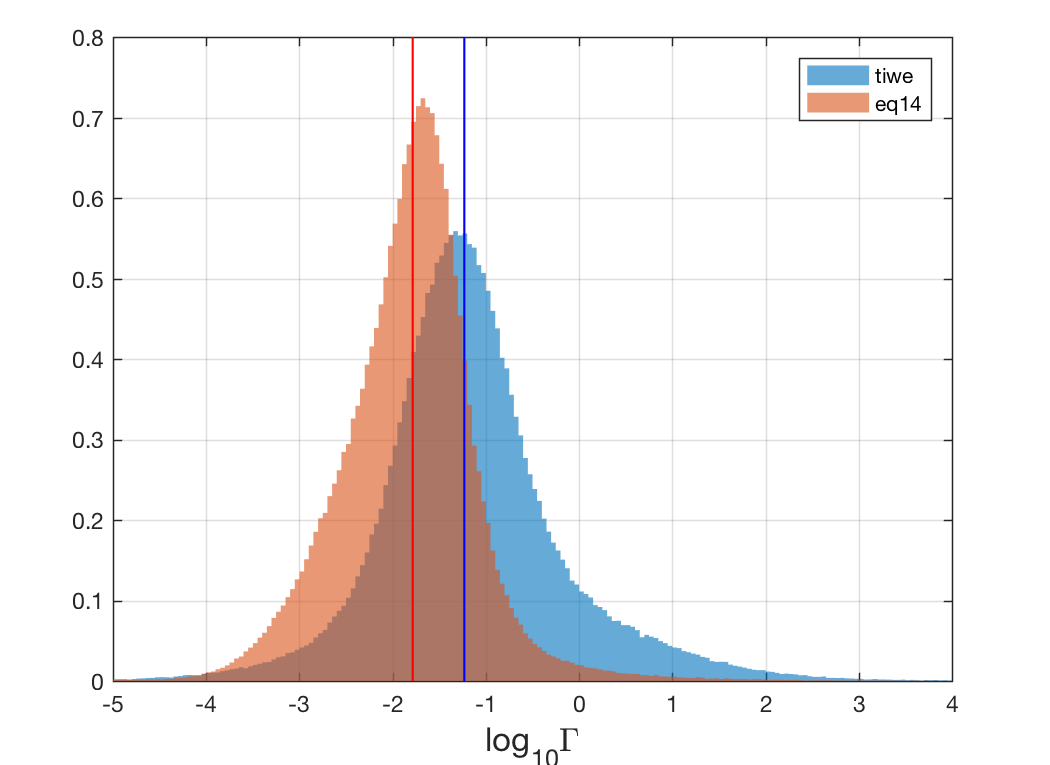
\includegraphics[scale=0.8]{tiwe_eq14_gamma_compare.png}
\caption{Histograms of gamma computed from combined TIWE data and EQ14 data (all data, not just patches).}
\label{tiwe_eq14_gamma_hist}
\end{figure}

\clearpage

\subsection{Patches}
Next I identify patches the same way in the tiwe data in \verb+Find_patches_TIWE_cham.m+.


\begin{figure}[htbp]
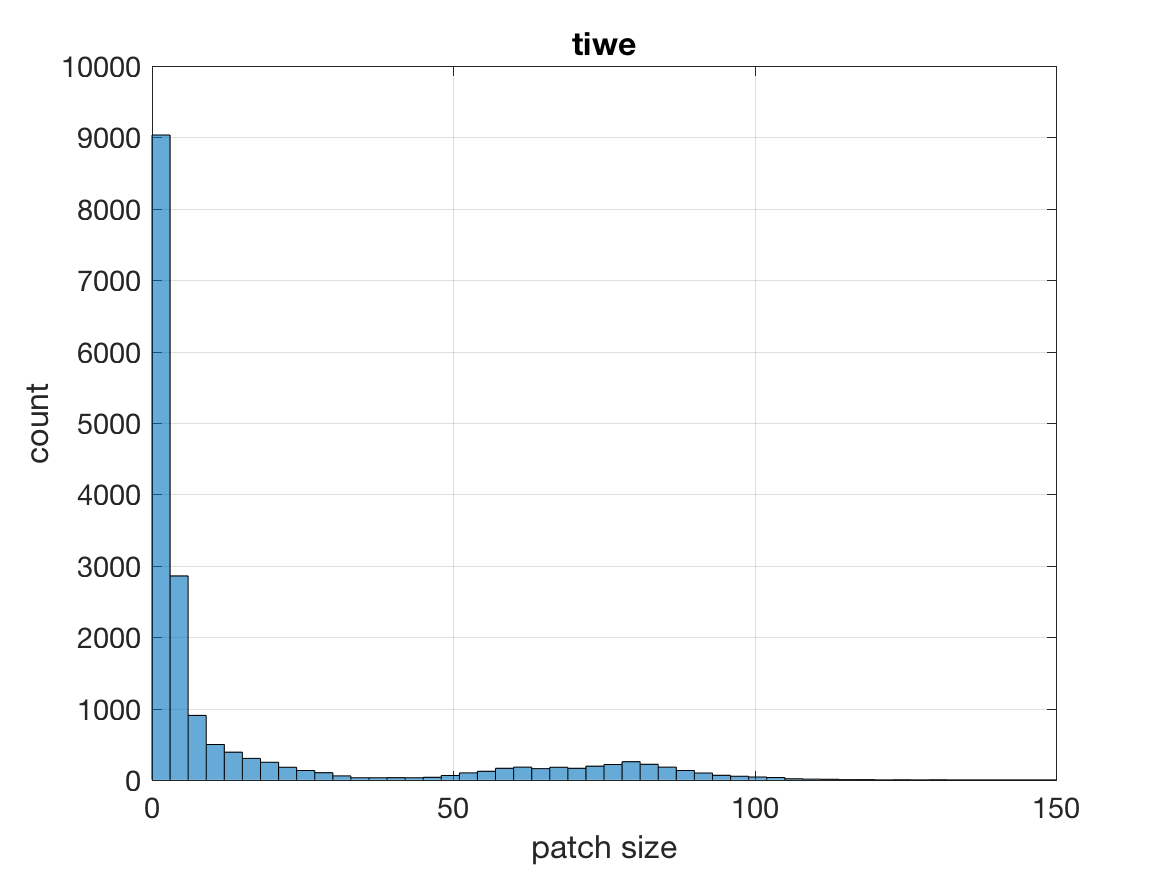
\includegraphics[scale=0.8]{tiwe_patchsize_hist.png}
\caption{Histograms of patch sizes from combined TIWE.}
\label{tiwe_patchsize_hist}
\end{figure}


\begin{figure}[htbp]
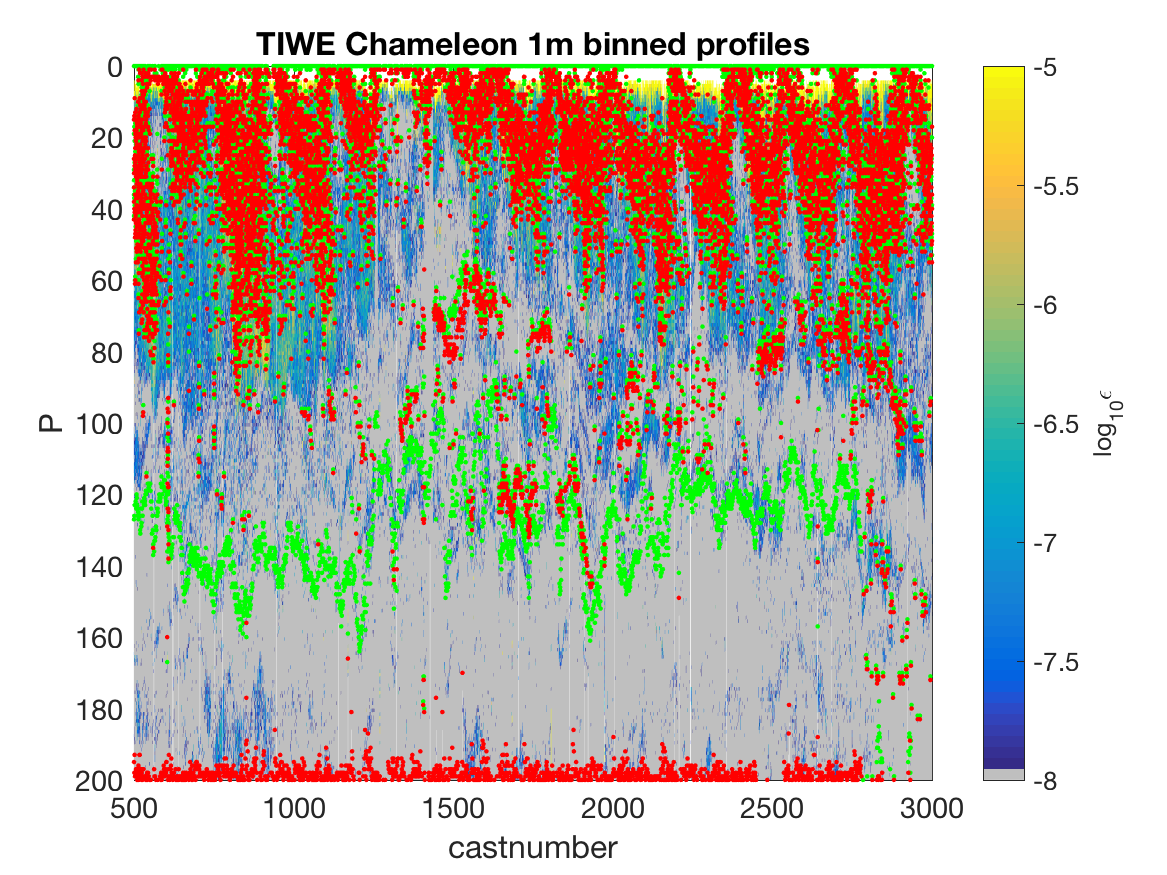
\includegraphics[scale=0.8]{tiwe_pcolor_wpatches.png}
\caption{patches  from combined TIWE.}
\label{tiwe_pcolor_patchs}
\end{figure}


\clearpage

Most of the really big patches are down below 150m where dtDz is weird. I'll exclude that data, and the surface mixed layer also.

\begin{figure}[htbp]
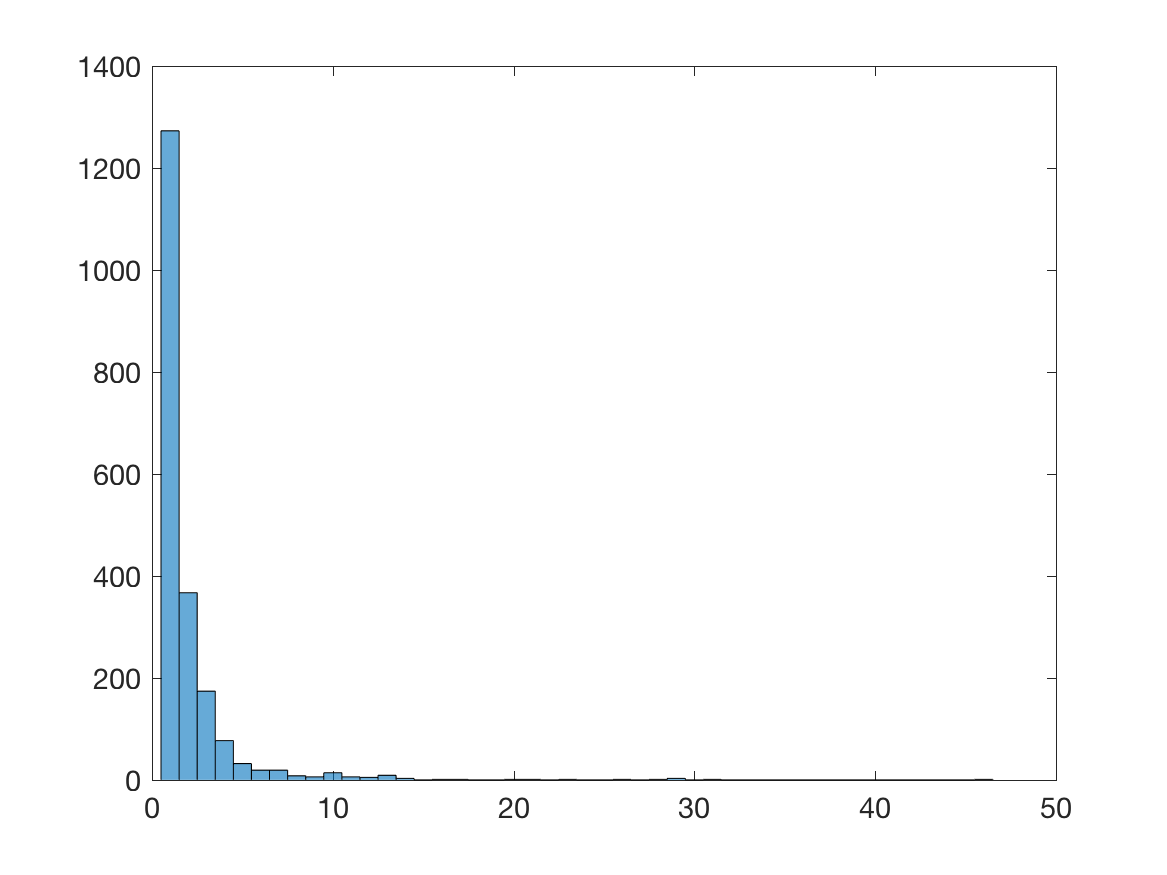
\includegraphics[scale=0.8]{tiwe_patchsize_mid_hist.png}
\caption{Histograms of patch sizes from combined TIWE.}
\label{}
\end{figure}


\begin{figure}[htbp]
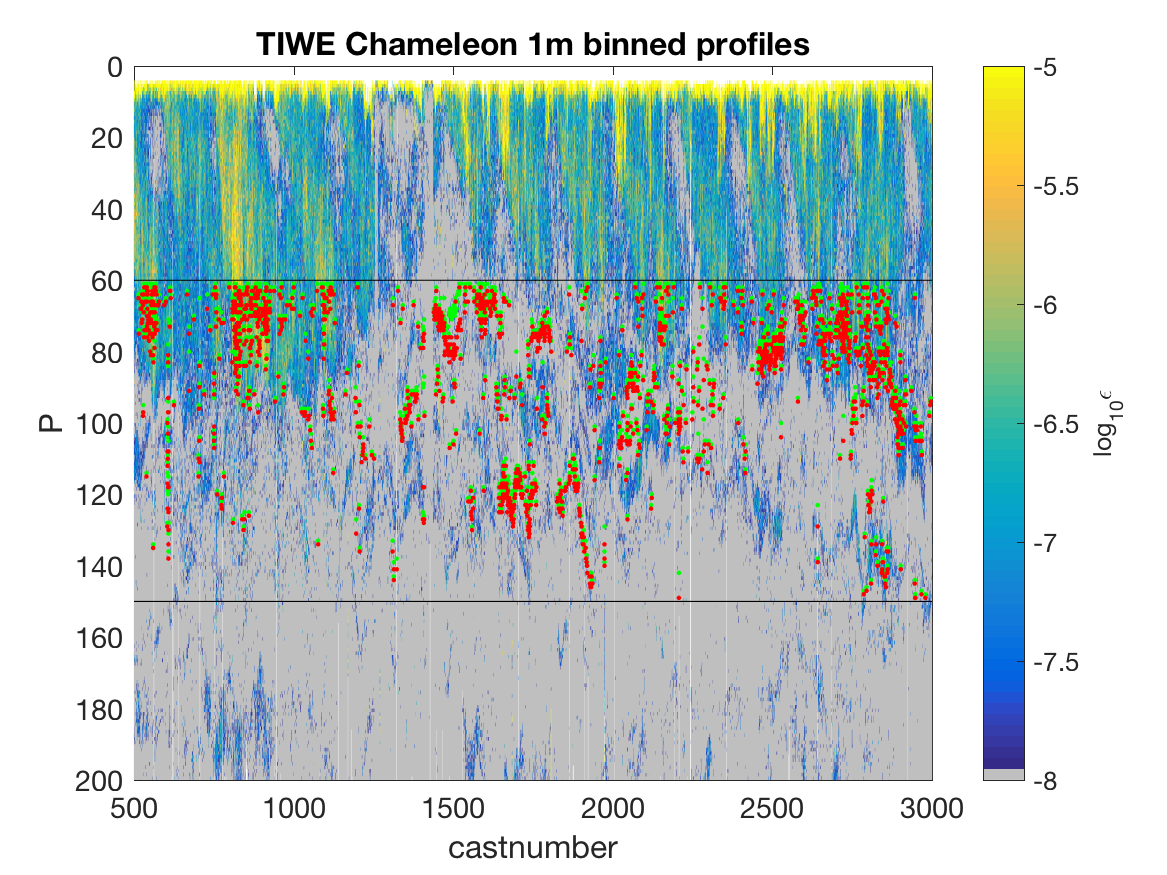
\includegraphics[scale=0.8]{tiwe_pcolor_wpatches_mid.png}
\caption{patches  from combined TIWE.}
\label{}
\end{figure}

\clearpage

\subsection{Gamma in patches}

Ok, first what does gamma look like if just use data within or near these patches?

\begin{figure}[htbp]
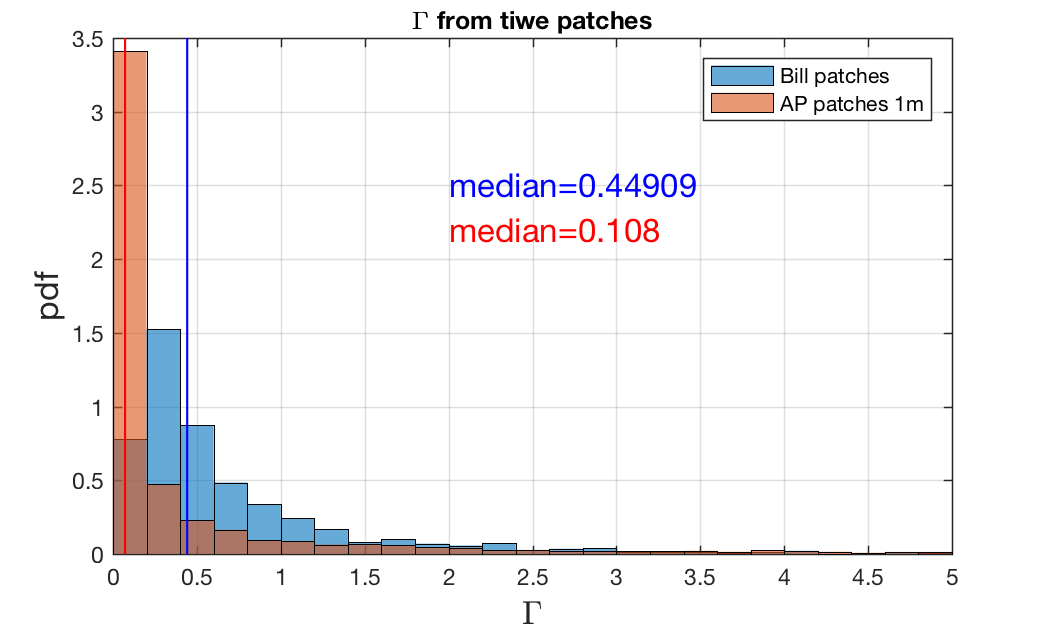
\includegraphics[scale=0.8]{tiwe_gam_billvsAP.png}
\caption{Gamma computed from tiwe patch data. My patches are from the 1m-binned profile data.}
\label{}
\end{figure}




\clearpage
%~~~~~~~~~~~~~~~~~~~~~~~~~~~~~~
\section{Identifying Patches from raw chameleon data}

I tried computing patches and gamma from the 1m averaged profiles, and still got a different gamma from Bill for tiwe. So next i'll try computing patches from the raw profiles instead of the averaged data. Eventually I should also compute n2,dtdz,chi, and eps from the raw data over each patch; before now i've just grabbed the 1m average data points within each patch.


First i'll experiment computing patches from the raw eq14 profiles and see how different they are from the patches I already computed with the 1m avg data.

See \verb+FindPatches_EQ14_Raw.m+.

My approach to doing this:
\begin{itemize}
\item Find patches \verb+FindPatches_EQ14_Raw.m+ ; this gives us the start and stop pressures for each patch in each profile
\item Next I want to compute N2,dT/dz,chi,eps over just these patches, instead of the usual evenly-spaced 1m bins (this is done in \verb+average_data_gen1.m+, which is called by a script like \verb+run_eq14.m+).
\item I am making a modifed version of \verb+average_data_gen1.m+ that takes the start/stop pressure of each bin as input instead of just making evenly spaced bins. My version is called \verb+average_data_PATCH_AP.m+
\item So I will run a modified version of \verb+run_eq14.m+ that loads the raw data, then calls \verb+average_data_PATCH_AP.m+, which will return an `avg' structure with data computed for each patch.
\end{itemize}






\end{document}  
